\documentclass[border=2pt]{standalone}
\usepackage[T1]{fontenc}
\usepackage{times}
\usepackage{pgfplots}
\usepgfplotslibrary{groupplots}
\pgfplotsset{compat=1.18}
\definecolor{cA}{HTML}{2A78D6}
\definecolor{cB}{HTML}{EB6834}
\definecolor{cC}{HTML}{1BAF7A}
\definecolor{cD}{HTML}{EDA100}
\definecolor{cGrey}{HTML}{6F7988}
\definecolor{cLight}{HTML}{AEB4BD}
\definecolor{cRule}{HTML}{D9DEE5}
\pgfplotsset{every axis/.append style={font=\footnotesize, axis line style={cGrey}, tick style={cGrey},
  major grid style={cRule, line width=0.3pt}, ymajorgrids, tick pos=left, label style={font=\footnotesize},
  title style={font=\footnotesize\bfseries, yshift=-2pt}, legend style={font=\scriptsize, draw=none, fill=none}},
  err/.style={error bars/.cd, y dir=both, y explicit, error mark options={rotate=90, mark size=1.5pt}, /pgfplots/.cd}}
\begin{document}
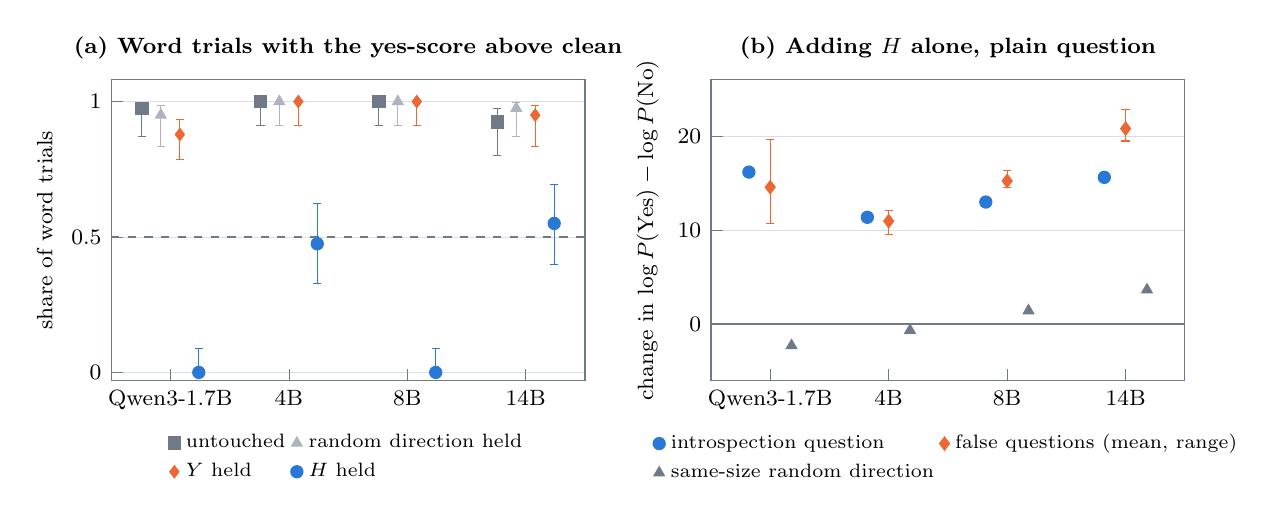
\begin{tikzpicture}
\begin{groupplot}[group style={group size=2 by 1, horizontal sep=1.6cm}, width=7.6cm, height=5.4cm, xtick={1,2,3,4}, xticklabels={Qwen3-1.7B,4B,8B,14B}, xmin=0.5, xmax=4.5]
\nextgroupplot[title={(a) Word trials with the yes-score above clean}, ymin=-0.03, ymax=1.08, ylabel={share of word trials},
  legend style={at={(0.5,-0.14)}, anchor=north, legend columns=2}, legend cell align=left]
\draw[cGrey, dashed, line width=0.5pt] (axis cs:0.5,0.5) -- (axis cs:4.5,0.5);
\addplot[only marks, mark=square*, mark size=2.2pt, color=cGrey, err] coordinates {(0.7600,0.97500) += (0,0.02057) -= (0,0.10381) (1.7600,1.00000) += (0,0.00000) -= (0,0.08762) (2.7600,1.00000) += (0,0.00000) -= (0,0.08762) (3.7600,0.92500) += (0,0.04916) -= (0,0.12364)};
\addlegendentry{untouched}
\addplot[only marks, mark=triangle*, mark size=2.2pt, color=cLight, err] coordinates {(0.9200,0.95000) += (0,0.03618) -= (0,0.11504) (1.9200,1.00000) += (0,0.00000) -= (0,0.08762) (2.9200,1.00000) += (0,0.00000) -= (0,0.08762) (3.9200,0.97500) += (0,0.02057) -= (0,0.10381)};
\addlegendentry{random direction held}
\addplot[only marks, mark=diamond*, mark size=2.2pt, color=cB, err] coordinates {(1.0800,0.87838) += (0,0.05630) -= (0,0.09364) (2.0800,1.00000) += (0,0.00000) -= (0,0.08762) (3.0800,1.00000) += (0,0.00000) -= (0,0.08762) (4.0800,0.95000) += (0,0.03618) -= (0,0.11504)};
\addlegendentry{$Y$ held}
\addplot[only marks, mark=*, mark size=2.2pt, color=cA, err] coordinates {(1.2400,0.00000) += (0,0.08762) -= (0,0.00000) (2.2400,0.47500) += (0,0.15003) -= (0,0.14565) (3.2400,0.00000) += (0,0.08762) -= (0,0.00000) (4.2400,0.55000) += (0,0.14295) -= (0,0.15171)};
\addlegendentry{$H$ held}
\nextgroupplot[title={(b) Adding $H$ alone, plain question}, ymin=-6, ymax=26, ylabel={change in $\log P(\mathrm{Yes})-\log P(\mathrm{No})$},
  legend style={at={(0.5,-0.14)}, anchor=north, legend columns=2}, legend cell align=left]
\draw[cGrey, line width=0.5pt] (axis cs:0.5,0) -- (axis cs:4.5,0);
\addplot[only marks, mark=*, mark size=2.2pt, color=cA] coordinates {(0.820,16.1875) (1.820,11.3750) (2.820,13.0000) (3.820,15.6250)};
\addlegendentry{introspection question}
\addplot[only marks, mark=diamond*, mark size=2.4pt, color=cB, err] coordinates {(1.0000,14.57812) += (0,5.10938) -= (0,3.89062) (2.0000,10.96875) += (0,1.15625) -= (0,1.46875) (3.0000,15.25000) += (0,1.12500) -= (0,0.75000) (4.0000,20.81250) += (0,2.06250) -= (0,1.31250)};
\addlegendentry{false questions (mean, range)}
\addplot[only marks, mark=triangle*, mark size=2.2pt, color=cGrey] coordinates {(1.180,-2.2812) (2.180,-0.6562) (3.180,1.4375) (4.180,3.6562)};
\addlegendentry{same-size random direction}
\end{groupplot}
\end{tikzpicture}
\end{document}
